\documentclass[11pt]{amsart}
\usepackage{amsmath}
\usepackage{amssymb}
\usepackage{tikz}

\begin{document}

	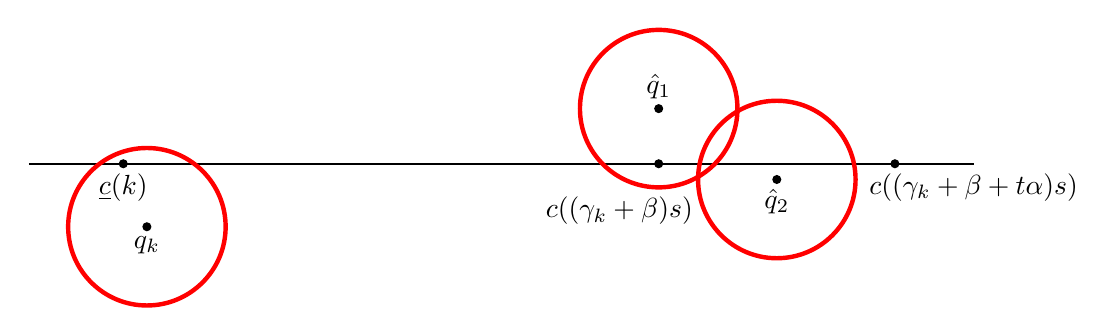
\begin{tikzpicture}
		\draw [thick] (-5,0) -- (7,0);
  \draw[fill] (-3.8,0) circle [radius=0.05];
  \node [below] at (-3.8,0) {$\underline c(k)$};
  \draw[fill] (3,0) circle [radius=0.05];
  \node [below] at (2.5,-0.3) {$c((\gamma_k+\beta)s)$};
   \draw[fill] (6,0) circle [radius=0.05];
  \node [below] at (7,0) {$c((\gamma_k+\beta+t\alpha)s)$};
\draw [red, ultra thick] (-3.5,-0.8) circle [radius=1];
  \draw[fill] (-3.5,-0.8) circle [radius=0.05];
  \node [below] at (-3.5,-0.8) {$q_k$};
  \draw [red, ultra thick] (3,0.7) circle [radius=1];
  \draw[fill] (3,0.7) circle [radius=0.05];
  \node [above] at (3,0.7) {$\hat q_1$};
  \draw [red, ultra thick] (4.5,-0.2) circle [radius=1];
  \draw[fill] (4.5,-0.2) circle [radius=0.05];
  \node [below] at (4.5,-0.2) {$\hat q_2$};
	\end{tikzpicture}

\end{document}